\documentclass[12pt,table]{article}

\usepackage[table]{xcolor}
% TEMPLATE DEFAULT PACKAGES
\usepackage{amssymb,amsmath,amsfonts,eurosym,geometry,ulem,graphicx,xcolor,setspace,sectsty,comment,natbib,pdflscape,array,adjustbox,threeparttable}

% ADDED PACKAGES FOR THIS MANUSCRIPT
\usepackage{palatino,newtxmath,multirow,titlesec,threeparttable,tabu,booktabs,titlesec,threeparttable,mathtools,bm,bbm,subcaption,pdflscape,tcolorbox,mathrsfs,float}
% endfloat,



%\usepackage{kbordermatrix}% http://www.hss.caltech.edu/~kcb/TeX/kbordermatrix.sty
%\usepackage{amsmath}% http://ctan.org/pkg/amsmath

\usepackage[colorinlistoftodos]{todonotes}

\usepackage{afterpage}
\usepackage[hyphens]{url}
\usepackage[margin=1cm]{caption}

\usepackage[draft]{hyperref}
\newcommand{\tim}{$\,\times\,$}
% FIGURES & TABLES CAPTION STYLING
\captionsetup[figure]{labelfont={bf},name={Figure},labelsep=period}
\captionsetup[table]{labelfont={bf},name={Table},labelsep=period}

% SECTION TITLE SETTINGS
\titlelabel{\thetitle.\enskip}
\titleformat*{\section}{\large\bfseries}
\titleformat*{\subsection}{\normalsize\bfseries}

% COLUMN TYPES
\newcolumntype{L}[1]{>{\raggedright\let\newline\\\arraybackslash\hspace{0pt}}m{#1}}
\newcolumntype{C}{>{\centering\arraybackslash}p{5.2em}}
\newcolumntype{D}{>{\centering\arraybackslash}p{5em}}
\newcolumntype{E}{>{\centering\arraybackslash}p{6em}}
\newcolumntype{F}{>{\centering\arraybackslash}p{4em}}

\newcolumntype{R}[1]{>{\raggedleft\let\newline\\\arraybackslash\hspace{0pt}}m{#1}}

\newcolumntype{J}{>{\raggedright\arraybackslash}p{5em}}
\newcolumntype{K}{>{\raggedleft\arraybackslash}p{5em}}
\newcolumntype{M}{>{\raggedleft\arraybackslash}p{6em}}

\renewcommand{\arraystretch}{1.2} 

\newcommand{\regtext}{
Standard errors are clustered at the small-area level (in parentheses).  The water service area is divided into 2,974 small-areas.
\textsuperscript{c} p$<$0.10,\textsuperscript{b} p$<$0.05,\textsuperscript{a} p$<$0.01 \,\,
}


% MARGINS AND SPACING
\normalem
\geometry{left=1.1in,right=1.1in,top=1.0in,bottom=1.0in}
\setlength{\parskip}{2.5pt}

% SPECIAL CELL 
\newcommand{\specialcell}[2][c]{%
	\begin{tabular}[#1]{@{}l@{}}#2\end{tabular}}

% NO INDENT ON FOOTNOTES
\usepackage[hang,flushmargin]{footmisc}

\begin{document}

\begin{titlepage} 
%\title{{Borrowing with Unpaid Bills}\thanks{}}
%\title{{Microcredit from Delaying Bill Payments}\thanks{}}
\title{Microcredit from Delaying Bill Payments}
\author{\\[3em]
  William Violette\thanks{Federal Trade Commission, Washington, DC. E-mail: william.j.violette@gmail.com   Any opinions and conclusions expressed herein are those of the author and do not necessarily represent the views of the Federal Trade Commission or its Commissioners.  Many thanks to Matthew Panhans, Miriam Larson-Koester, Adrian Rubli-Ornelas, and Stefano Polloni.} \\
 \\ 
  }
\vspace{30mm}
\date{\vspace{5mm}This Version: \today}
\maketitle
\begin{abstract}

Delaying bill payments to public utilities may provide an important strategy for households with volatile incomes to smooth their consumption.  At the same time, tolerating late payments may reduce net revenues for utilities, which often leads to higher prices to cover costs.  Using billing records from a large water utility in Manila, this paper estimates a household consumption and savings model to evaluate counterfactual payment policies.  A popular proposal to ensure upfront payments --- prepaid metering --- recoups less revenue than is needed to compensate households for their loss of consumption smoothing.  Alternatively, a revenue-neutral policy allowing more late payments increases welfare by encouraging greater consumption smoothing.



\vspace{1in}
\textbf{Keywords:} credit constraints; consumption smoothing; water utilities. \\
\textbf{JEL Codes:} O13; E21; L95. \\
\bigskip
\end{abstract}
\setcounter{page}{0}
\thispagestyle{empty}
\end{titlepage}
\pagebreak \newpage

%\spacing{1.5}
\onehalfspacing

\section{Introduction}

Key notes to fill in later:
- Ignore externalities of booster pumps
- No quantity margin because of splitting of taps and because census data indicates really high coverage
- Reweight by household number
- Also measure by closest pipe for robustness


\section{Data}

Section: Data

	- only households connected earlier (explain) (what share are those?!)
	- consumption per HH
	- reweight data for household level?!

	- Put in a table describing pipe-replacement;  describe staggered approach; predict pipe-replacement?

Consumption is measured according to average consumption for not-shared households!  What extra assumption is that!!!  NEED ROBUSTNESS!!! 

MEASURING AVERAGE PRICES


\section{Descriptives}

Descriptive evidence indicates that fixing pipes improves water pressure, quality, and reliability, which may each affect consumer welfare.  Table~\ref{table:descriptives} tracks water service improvements by comparing average household survey responses before and after pipe replacement.   [summarize the findings]

Consumers also invest in products and behaviors to compensate for low piped water service quality.  These investments help reveal which aspects of piped water service are most valuable to consumers as well as most affected by pipe replacement.  

Large investments in booster pumps suggest that households strongly value water pressure.  Booster pumps are both expensive to purchase and operate. In Manila, booster pumps range in price from 1,200 to 15,000 PhP, which represents a large expense given average monthly household incomes of 26,023PhP.\footnote{Figures come from scraping results from the first page of searching ``booster pumps'' on the popular online marketplace in Manila, \url{https://www.lazada.com.ph/},  yielding 22 entries with horsepower listed.  Median monthly household income is computed for Metro Manila using the 2015 Family Income and Expenditure Survey.}  The median booster pump uses a 0.75 horsepower engine, which generates monthly costs of around 405 PhP at prevailing energy prices.\footnote{A 1 horsepower engine uses around 0.786 Kw per hour.  Table~\ref{table:descriptives} indicates that households use their booster pumps for 2.6 hrs per day, which implies around 78 hours per month.  In 2012, tariffs for the electricity utility in Manila averaged around 8.8 PhP per KwH.}   Before pipe replacement, 40\% of households invest in booster pumps that increase water pressure.  After pipe replacement, the share of households using booster pumps drops to 15\%.  This finding is consistent with booster pumps providing an important substitute to pressure from new water pipes.

Small investments in water filters combined with frequent purchases of filtered water both before and as well as after pipe replacement indicate that households may not derive large benefits from improvements in piped water quality.  Only 12\% of households use water filters both before and after pipe replacements.  Low filter usage may stem from the fact that less than half of households report drinking from the tap while over 70\% of households report purchasing filtered water from local water-refilling stations.  These behaviors remain constant after pipe replacements.  Taken together, these findings indicate that water quality improvements from pipe replacements may not be primary drivers of changes in household welfare.

Households cope with unreliable water supply by investing in water storage tanks.  Before pipe replacement, 43\% of households report using water storage tanks.  This percentage only drops to 36\% following pipe replacement, which is consistent with households continuing to report frequent water outages even after pipe replacement.  While households seems to value reliable service, small changes in storage tank use suggest that reliability improvements are unlikely to account for a large share of the welfare gains from pipe replacements.

\begin{table}[h!] 
\centering
\caption{Average Survey Responses Before and After Pipe Replacement}\label{table:descriptives}
\vspace{-2mm}
\begin{threeparttable}
\begin{tabular}{@{}l*{1}{KKK}@{}}
\toprule
  & Before & After  & All \\
\midrule
Piped Water Service Quality \\[.5em]
\hspace{1em}$\text{Water has strong pressure (6pm-12am)}^{\dagger}$ & 0.26 & 0.56 & 0.48 \\
\hspace{1em}$\text{Water has no pressure (6pm-12am)}^{\dagger}$  & 0.29 & 0.04 & 0.09 \\
% \hspace{1em}$\text{Hours with pressure per day}^{\dagger}$ & 21.40 & 23.39 & 22.48 \\
\hspace{1em}Water interruptions in last 3 months & 2.28 & 1.93 & 2.13 \\
\hspace{1em}Water has foreign bodies & 0.23 & 0.05 & 0.14 \\
\hspace{1em}Water is discolored & 0.08 & 0.03 & 0.04 \\
\hspace{1em}Water has unusual taste/smell & 0.12 & 0.03 & 0.05 \\
\\[-.5em]
Household Service Quality Investments \\[.5em]
\hspace{1em}Has booster pump & 0.37 & 0.11 & 0.16 \\
\hspace{1em}Hours booster pump is used per day & 2.86 & 2.47 & 2.51 \\
\hspace{1em}Has water storage tank & 0.43 & 0.36 & 0.39 \\
\hspace{1em}Has water filter & 0.12 & 0.12 & 0.11 \\
\hspace{1em}Purchases filtered water & 0.68 & 0.74 & 0.69 \\
\hspace{1em}Purchases from a deepwell & 0.05 & 0.02 & 0.03 \\
\hspace{1em}Spending on non-piped water (PhP) & 90.93 & 88.26 & 86.99 \\
\hspace{1em}Drinks from the tap & 0.50 & 0.46 & 0.52 \\
% \hspace{1em}Boils tap water before drinking & 0.23 & 0.19 & 0.21 \\
\\[-.5em]
Demographics \\[.5em]
\hspace{1em}Household size & 4.91 & 4.94 & 4.96 \\
\hspace{1em}Employed members & 1.57 & 1.36 & 1.47 \\
\hspace{1em}High-skilled employment & 0.11 & 0.09 & 0.10 \\
\hspace{1em}Lives in duplex& 0.25 & 0.29 & 0.26 \\
\hspace{1em}Lives in single house& 0.55 & 0.51 & 0.57 \\
\hspace{1em}Other households sharing tap& 0.86 & 0.88 & 0.91 \\
\\[-.5em]
Households & 13,441 & 8,461 & 57,018 \\
\bottomrule
\end{tabular}
\begin{tablenotes}
\footnotesize
\item  $\dagger$ when not using booster pump.  Bill, Unpaid Balance, Payment, and Income are in PhP.  Measures exclude months where households remain disconnected through the end of the sample period.  Billing data include households for household-month observations.  Income data include households for household-month observations.  45 PhP = 1 USD \,\,
% See Appendix~\ref{appendix:sampleconstruction} for more details on the sample construction.
\end{tablenotes}
\end{threeparttable}
\end{table}


Increases in water pressure from pipe replacements may lead households to increase their monthly water consumption.  Rapid water flow allows households to complete a greater number of water-using activities like cleaning and bathing in the same amount of time.  Greater water pressure may also allow households to engage in new activities that require minimum pressure levels such as showering.\footnote{By contrast, water quality improvements may have an ambiguous effect on water consumption.  On one hand, cleaner water may induce households to use more tap water for cooking and cleaning.  On the other hand, cleaner water may increase the productivity of cleaning and bathing, which may lead households to use less piped water.}  Figure~\ref{figure:pipecons} plots average monthly water usage per household in the 4 years before and 6 after pipe replacement.  Usage increases from an average of 18.5m3 before pipe replacement to 24.7m3 after pipe replacement, which represents an 18\unskip\% increase.  The increase in usage occurs abruptly at the year of pipe replacement and remains at roughly the same level in the following 6 years.  This sustained increase in consumption suggests that pipe replacement may provide sustained impacts on household welfare.  

The absence of strong pre-trends in usage suggests that replacement projects are not targeted to areas with particular trends in local water demand.  Instead, this pattern is consistent with the company's stated goal of sequentially replacing old pipes according to engineering specifications.  Table~\ref{table:descriptives} further supports this theory by indicating few demographic differences between households that receive pipe replacement projects (columns (1) and (2)) and all households (column (3)).  Also, demographic characteristics appear relatively similar before and after pipe replacement, which suggests that pipe replacements were not coupled with other policies that may have also affected demand for water.  

\begin{figure}
\begin{center}
\caption{Average Consumption per Household with Years to Pipe Replacement}\label{figure:pipecons}
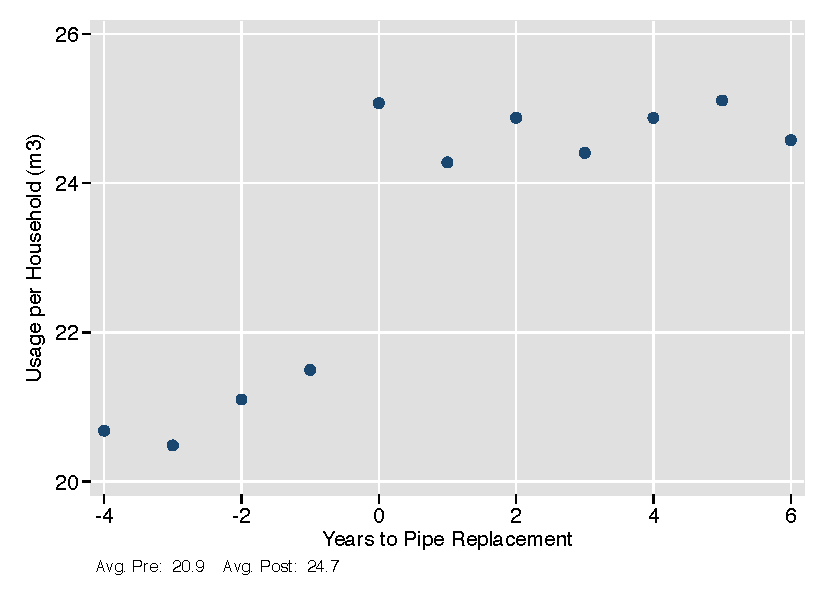
\includegraphics[scale=1]{tables/pipe_cons.pdf}
\end{center}
%%% add counts and average change in discussion
\end{figure}
% discuss dynamics!!! of figure!!

Mapping these increases in consumption into household welfare requires measuring how households trade off water usage and price.  Prices are determined by the government regulator who imposes an increasing tariff schedule according to monthly usage, which is standard among public utilities (\cite{hoque2013state}).  Despite steep increases in marginal price at specific levels of usage, households do not appear to be sensitive to these price changes because households are not observed adjusting their consumption strategically to avoid higher prices (cite appendix).  The regulator also increases prices gradually over time to ensure that the company continues to cover operating costs.  Since households also gradually increase their average usage over this interval, it is unclear whether households are responsive to these price increases (cite appendix).

The government regulator also gives the water company discretion to assign households to a high-price tariff schedule if they have any business activity at their residence, which provides a novel source of price variation in the context of public utilities.  In the vast majority of cases, the high price tariff is applied to households that operate small food stands (or ``Sari-Sari'' stores).  For a household with average monthly usage, the high-price tariff results in an average price of 26.4PhP/m3 while the regular tariff results in an average price of 20.5PhP/m3 (cite appendix for tariff).  The water company periodically visits consumers and updates prices according to the activities observed at each consumer's residence.  In some cases, consumers request price changes, which prompts the company to investigate the household and determine the appropriate price.  Table~\ref{table:pricechangestatistics} provides average characteristics of households that are always observed with the regular price (in column (1)), that are always observed with the high price (in column (2)), and that are observed changing prices during the sample (in column (3)).  While the 2,442 households that experience price changes use more water than other households, they share similar demographic characteristics, which suggests that they may also share similar price-sensitivities.  

Figure~\ref{figure:usagepricechanges} plots average usage 4 years before and after households are switched from the regular price to the high price (in red) as well as before and after households are switched from the high price to the regular price (in blue).  Before the price change, average usage for both groups follows relatively constant trends.  The price change is associated with a usage jump for households switched to the regular price and a corresponding usage slide for households switched to the high price.  The changes in consumption appear relatively persistent up to 4 four years after the price changes.  These patterns indicate that household water usage is sensitive to large, discrete price changes.  


\begin{table}[h!] % PUT IN DEMOGRAPHICS PLEASE ?!?!?
\centering
\caption{Average Household Characteristics by Prices Charged}\label{table:pricechangestatistics}
\vspace{-2mm}
\begin{threeparttable}
\begin{tabular}{@{}l*{1}{KKK}@{}}
\toprule
  & Always Reg. Price & Always High Price  & Change Price \\
\midrule
Usage per Household (m3)& 19.95 & 20.17 & 23.42 \\
Household size & 4.98 & 4.74 & 4.99 \\
Employed members & 1.49 & 1.40 & 1.44 \\
High-skilled employment & 0.09 & 0.06 & 0.06 \\
Lives in duplex& 0.26 & 0.26 & 0.26 \\
Lives in single house& 0.50 & 0.59 & 0.54 \\
Other households sharing tap& 0.90 & 0.92 & 0.95 \\
\\[-.5em]
Households & 43,442 & 3,823 & 2,442 \\
\bottomrule
\end{tabular}
\begin{tablenotes}
\footnotesize
\item  Reg. refers to regular price.  

Pressure is 6 to midnight! Bill, Unpaid Balance, Payment, and Income are in PhP.  Measures exclude months where households remain disconnected through the end of the sample period.  Billing data include households for household-month observations.  Income data include households for household-month observations.  45 PhP = 1 USD \,\,
% See Appendix~\ref{appendix:sampleconstruction} for more details on the sample construction.
\end{tablenotes}
\end{threeparttable}
\end{table}

\begin{figure}
\begin{center}
\caption{Usage and Price Changes}\label{figure:usagepricechanges}
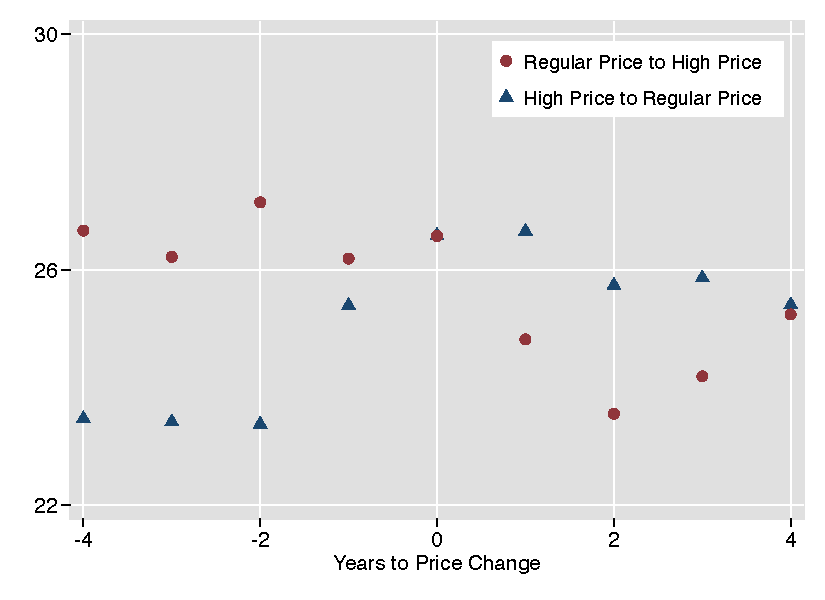
\includegraphics[scale=1]{tables/r_to_s_graph.pdf}
\end{center}
\end{figure}

\section{Model}

A simple model of household water demand connects changes in water usage to changes in household welfare as a result of pipe replacements.  In this model, households choose their monthly water usage as well as whether to use a booster pump to boost water pressure.  

Each month, household utility takes the following form
\begin{align}
\label{eq:utility}
U\,=\,\frac{1}{\alpha} \, \Big[ \,  ( \theta_1 B \, +  \, \theta_2 R + \, \theta_3 B R ) \,  w  \, -\, \frac{1}{2}(w - \gamma + \epsilon)^2 \, \Big] \, + \, x
\end{align}
where $w$ is water consumption and $x$ represents a bundle of all other goods consumed by the household.  Water service quality is captured by $( \theta_1 B \, +  \, \theta_2 R + \, \theta_3 B R )$ where $B$ equals 1 if the household uses a booster pump (and zero otherwise) and $R$ equals 1 after pipe replacement (and zero otherwise).  The $\theta$ terms capture the household's preference for water service quality from booster pumps, pipe replacements, and the combination of the two.  For example, $\theta_3<0$ implies that booster pumps and pipe replacements are substitutable in producing water service quality.  Water service quality enters multiplicatively with water consumption, which nests the assumption that each unit of water consumption is affected equally by water service quality.  $\alpha$ reflects price sensitivity, and $\gamma$ reflects the satiation amount of water usage.  $\epsilon$ captures idiosyncratic monthly variation in satiation water usage such as changes in weather or in the number of household members using water.  $\epsilon$ is assumed to follow a normal distribution with zero mean and standard deviation $\sigma_{\epsilon}$.  This approach assumes that preferences for water are quasi-linear, which implies that water consumption does not depend on household income [ back this up with more evidence? ].  

Households maximize utility subject to the following budget constraint
\begin{align}
\label{eq:bc}
p\,w \,+\, x \, + (F + \upsilon) B \, = y 
\end{align}
where $p$ is the average price of water while the price of all other goods, $x$, is normalized to 1.  This approach includes the simplifying assumption that households respond to a single, average water price $p$ despite facing marginal prices that increase with monthly consumption.  This assumption is consistent with descriptive evidence that households appear unresponsive to marginal prices (cite appendix).   $F$ is total cost of renting and using a booster pump each month.  This approach assumes that Manila has a competitive market for renting/selling booster pumps.  $\upsilon$ captures idiosyncratic monthly variation the booster pump cost such as changes in the electricity price or variation in installation costs. $\upsilon$ is assumed to follow a normal distribution that is assumed to be uncorrelated with $\epsilon$ and has zero mean and standard deviation $\sigma_{\upsilon}$.  $y$ is monthly household income.  

% as well as other research on public utility price responsiveness (\cite{ito2014consumers}, and the water ito paper?).  

Maximizing household utility in equation $(\ref{eq:utility})$ subject to the budget constraint in equation $(\ref{eq:bc})$ for a given choice of booster pump usage, $B$, yields the following expression for monthly water demand
\begin{align}
w^{*} \, = \, \gamma \, - \, \alpha p +  \theta_1 B \, + \, \theta_2 R  \,+ \, \theta_3 B R \,  + \, \epsilon
\end{align}
Water demand depends linearly on the satiation preference, $\gamma$, as well as price, booster pump use, and pipe repairs.  Given optimal water demand, $w^{*}$, households can then choose whether to use a booster pump by comparing expected utilities with and without booster pumps.  Households use booster pumps when the following expression is greater than zero
\begin{align}
E\Big[ \,V_{B=1 - B=0}^{*}\,\Big]  = (\theta_1 + \theta_3 R) \Big(  \frac{\theta_1 + \theta_3 R}{2\alpha} + \frac{\gamma +  \theta_2 R}{\alpha} - p  \, \Big) \, - \, (F \, + \upsilon)
\end{align}
% Since $\epsilon$ is assumed to be  normal, it falls out of the equation
When booster pumps increase service quality $\theta_1>0$, booster pump use is increasing in household's fixed water preference, $\gamma$, and decreasing in the water price, $p$.  Booster pump use decreases following pipe replacements if $\theta_3$ is sufficiently negative.  

Given booster pump demand, the probability of observing a household choose to use a booster pump, $B^{*}$ can be expressed as follows
\begin{align}
Pr[B^{*}=1] \,\, = \,\, \Phi\Bigg( \, \frac{ (\theta_1 \theta_2 + \theta_1 \theta_3 + \theta_2 \theta_3) R + \frac{1}{2}(\theta_1^2 + \theta_3^2)  + \gamma (\theta_1 + \theta_3 R) \Big] - (\theta_1 + \theta_3 R) p \, - \, F }{\sigma_{\upsilon}} \, \Bigg)
\end{align}
where $\Phi(.)$ is the cumulative distribution function of the standard normal distribution.  Conditional on booster pump use, the probabilities of observing households use a particular amount of water, $w^{obs}$, can be expressed as follows
\begin{align}
Pr[w^{*}=w^{obs} \,|\, B^{*}=1] \,\, &= \,\, \frac{1}{\sigma_{\epsilon}} \phi\Bigg( \, \frac{ w^{obs} - (\gamma \, - \, \alpha p +  \theta_1  + \, \theta_2 R  \,+ \, \theta_3 R )}{\sigma_\epsilon} \, \Bigg) \\
Pr[w^{*}=w^{obs} \,|\, B^{*}=0] \,\, &= \,\, \frac{1}{\sigma_{\epsilon}} \phi\Bigg( \, \frac{ w^{obs} - (\gamma \, - \, \alpha p \, + \, \theta_2 R   )}{\sigma_\epsilon} \, \Bigg)
\end{align}
Combining these expressions, the log-likelihood of observing each pair of booster pump use and water use across households, $i$, is as follows
\begin{align}
\begin{split}
LL = \sum_i & \mathbbm{1}\{ B^{obs}_i = 1 \} \,\Big[ \ln\big( Pr[B^{*}=1] \big) + \ln\big( Pr[w^{*}=w^{obs}_i \,|\, B^{*}=1] \big) \Big] \, + \\
 & \mathbbm{1}\{ B^{obs}_i = 0 \} \,\Big[ \ln\big( 1- Pr[B^{*}=1] \big) + \ln\big( Pr[w^{*}=w^{obs}_i \,|\, B^{*}=0] \big) \Big] 
 \end{split}
\end{align}


\section{Empirical Specification and Identification}

% ($\gamma, \alpha, \sigma_{\epsilon}$) ($\theta_2$)  ($\theta_1, \theta_3$) ($\sigma_{\upsilon}$)
The estimation recovers preferences for water, preferences for water service quality, as well as booster pump effectiveness and cost variability.

Fixed preferences for water, $\gamma$, are allowed to vary according to six demographic characteristics: household size, number of employed household members, whether the head of household has high-skilled employment, whether the household is ever assigned a high water price, and whether the household ever receives pipe replacement, as well as indicators for calendar months.\footnote{Preferences do not depend on time because usage does not exhibit strong trends over time.}  Fixed preferences are identified primarily from average usage levels for each demographic group. Month indicators capture seasonality in water demand, and year indicators capture how water preferences evolve over time.  Monthly variation in water usage identifies variation in fixed preferences, $\sigma_{\epsilon}$.

Since calendar month indicators absorb all of the time-series variation in price schedules, price sensitivity, $\alpha$, is identified primarily through household changes in usage as the company switches households between regular and high average prices.  This approach relies on the assumption that switching between prices is not correlated with other factors that may affect demand.  For example, households may increase their water demand as they open a roadside food-stand and switch to the high price.  Conversely, households that close their roadside food-stand may decrease their consumption at the same time as they are switched to the low price.  Both cases suggest that this approach would underestimate household price sensitivities.  

Both cases would also likely predict strong pre-trends in usage for the years leading up to price changes.  Figure~\ref{figure:usagepricechanges} plots usage pre-trends providing little evidence of salient trends before price changes.  Appendix Table~\ref{table:usageregs} further finds that the correlation between price and household usage remains stable after controlling for household demographics, small-area fixed effects, or household fixed effects.  This approach also assumes that price sensitivities identified for households that switch prices are representative of the full population of households.  Table~\ref{table:pricechangestatistics} provides some support for this assumption by finding broadly similar demographics across households exposed to different prices.  

Preference for water service quality from pipe replacements, $\theta_2$, is identified by the change in usage observed before and after pipe replacements.  Identification of $\theta_2$ requires assuming that this change in consumption can be entirely attributed to pipe replacements and not to changes in other factors that may affect household demand for water at the same time.  One concern may be that pipe improvements are paired with other infrastructure investments that drive increases in local income, population, and water demand.  Alternatively, the water company may strategically target pipe improvements to either boost areas with declining demand or accelerate areas with growing demand.  Figure~\ref{figure:pipecons} traces a sharp break in average usage at the year of pipe replacement with little evidence of strong trends before or after replacement projects.  These patterns are consistent with company reports that pipe replacements were not explicitly linked to other infrastructure projects and were instead planned primarily to minimize engineering costs.

Preferences for booster pumps before pipe replacement, $\theta_1$, and after pipe replacement, $(\theta_1+\theta_3)$, are identified both from cross-sectional differences in usage for households with and without booster pumps as well as from changes in booster pump usage before and after pipe replacement projects.  Identification requires assuming that booster pump use accounts for all of the average differences in usage between households with and without booster pumps after conditioning on households' observable characteristics and pipe replacement status.  This assumption may not hold if households choose to use booster pumps to cope with unobserved variation in water service quality specific to their neighborhoods.  To partially test this assumption, Appendix Table~\ref{table:boosterregs} finds that the positive correlation between water use and booster pump use remains stable even after controlling for calendar month fixed effects as well as small-area fixed effects, which may both capture local variation in water service quality.

Identification of booster pump preferences also requires assuming that changes in booster pump use before and after pipe replacement projects are driven entirely by these projects and not by any other factors such as shifts in water preferences that may also be correlated with these projects.  Appendix Table~\ref{table:boosterregs} finds that the negative correlation between booster pump use and pipe replacement projects remains stable after accounting for household demographics and small-area fixed effects.  

This approach also assumes that booster pumps do not impose substantial negative externalities on local water service quality.  A recent engineering literature has raised the possibility that booster pumps interfere with water flow in pipe mainlines, reducing pressure along the entire pipe (\cite{taylor2014reducing}).  However, this problem may not be as salient in the context of Manila.  The water company has not raised booster pumps as a policy problem in any of their internal documents.\footnote{Booster pumps are sometimes mentioned in water company investigations of consumer complaints as an explanation for household water pressure and never as problem to be addressed.}  Moreover, externalities would predict large water usage gaps between those with and without booster pumps in the same neighborhood.  By contrast, Table~\ref{table:usageregs} finds a similar association of booster pump use and water usage with and without small-area fixed effects.   % Taken together, the empirical evidence is supportive of the relatively strong assumptions necessary to identify booster pump preferences.

While fixed monthly costs of booster pumps, $F$, are calibrated to equal the expected monthly cost of operating a booster pump, the estimation strategy recovers the distribution of these costs, $\sigma_{\upsilon}$, that best matches the observed shares of households using booster pumps.  Identification of $\sigma_{\upsilon}$ requires the assumption that cost variation, $\upsilon$, is uncorrelated with taste variation, $\epsilon$.  This assumption implies that after accounting for observed demographic and other factors, differences in booster pump use are entirely driven by unobserved costs rather than unobserved preferences.



\section{Results}




\begin{table}[h!] 
\centering
\caption{Structural Estimates}\label{table:estimates}
\vspace{-2mm}
\begin{threeparttable}
\begin{tabular}{@{}l*{1}{c}@{}}
\toprule
  &  (1)   \\
\midrule
Fixed Preferences & \\
\hspace{1em}Intercept & 13.31
 \\
 						& (0.000
) \\
\hspace{1em}Household Size & 3.01
 \\
 							& (0.000
) \\
\hspace{1em}Employed Household Members & 0.48
 \\
 						& (0.000
) \\
\hspace{1em}High Skill Employment & 2.04
 \\
 						& (0.000
) \\
\hspace{1em}Ever High Price & 4.12
 \\
 						& (0.000
) \\
\hspace{1em}Pipe Replacement Area & -0.55
 \\
 						& (0.000
) \\[.5em]
Price Sensitivity & 0.384
 \\
 						& (0.000
) \\[.5em]
Service Quality Preferences & \\
\hspace{1em}Post Replacement & 0.79
 \\
 						& (0.00
) \\
\hspace{1em}Booster Use & 3.27
 \\
 							& (0.00
) \\
\hspace{1em}Post Replacement $\times$ Booster Use & 0.54
 \\
 						& (0.00
) \\[.5em]
Usage Variability & 14.7
 \\
 						& (0.00
) \\[.5em]
Booster Cost Variability & 312.4
 \\
 						& (0.00
) \\
\bottomrule
\end{tabular}
\begin{tablenotes}
\footnotesize
\item This table predicts usage per household with pipe replacement, booster pump use, and price with different fixed effects.   \regtext 45 PhP = 1 USD \,\,
\end{tablenotes}
\end{threeparttable}
\end{table}







Need to fix the weighting of the estimates!!!!!!!!






Section Estimation:
	- show what happens when boosters are turned off


Section Welfare:
	- Welfare benefits with 10 yr 5\% loans (assume discount rates) or 50 yr 5\% loan?
	- Welfare benefits with cash
	- Are households willing to pay for pipe improvements?


Robustness:
	- Use nearest pipe replacement definition (selection into meter identification)



% - Discusses use of booster pumps in Clean Water Act 2004:  https://www.manilatimes.net/2018/11/04/legal-advice/dearpao/use-of-booster-pumps/461829/  http://r12.emb.gov.ph/ra-9275-the-philippine-clean-water-act/
% - https://idl-bnc-idrc.dspacedirect.org/bitstream/handle/10625/14878/108376.pdf?sequence=5
% - illegal booster pumps :  Consequence of El Niño 1997-98 on Manila water resources: new perspectives in water shortage management
% - seizing booster pumps : https://timesofindia.indiatimes.com/city/navi-mumbai/booster-pumps-used-by-some-socs-leading-to-water-crunch/articleshow/68856763.cms , https://timesofindia.indiatimes.com/city/nagpur/215-booster-pumps-seized/articleshow/69804589.cms




 % If households were sensitive to price increases at specific consumption levels, then households would be expected to frequently consume just below these levels.  However, Appendix Figure plots the frequency 






% The welfare benefits of fixing water pipes depends on which dimensions of service quality are improved by pipe replacement.  Table~\ref{table:descriptives} compares average household survey responses before and after pipe replacement.

% Allow services that they couldn't before

% Before pipe replacement, households experience weak water pressure and low water quality.  30\% of households report generally having no water pressure from 6 pm to 12 am in the absence of an extra household pump to boost water pressure.  23\% of households report that their piped water generally has foreign bodies.

% To compensate for low piped water quality, many households invest in private water booster pumps, storage drums, water filters, and purchases of non-piped water.  

% Both pressure and water quality improve substantially following pipe replacement.  The shares of households reporting no water pressure, water discoloration, foreign bodies, and unusual tastes/smells all drop to below 6\%.  

% - Quality complements more consumption
% - Water quality implies that consume the same, just enjoy it wayyy more
% 	- maybe need to clean things longer
% 	- maybe clean things the same but get way more utility

% - Pressure implies that quantity is positively linked to quality!
% 	- has the same feature?
% 	- use the same water, just less time...
% 	- costly to push for that extra water..... from a time perspective
% 		- Natural to think of relieving the pressure as leading to greater consumption!




	% Table: 
	% 	(A) What does pipe fixing mean?
	% 		- Quality, Hours, Flow

	% 	(B) How do households change their investments?

	% 	(C) How do households use their water?

	% 	(D) Household demographics including sharing
	% 		* N 
	% 	(E) Household consumption/payments/disconnection/standard deviation! (from billing data N)
	% 		* N




%%%% PIPE AGE %%%  possibly lower quality as well
% http://www.mayniladwater.com.ph/news-article.php?id=656
% West Zone concessionaire Maynilad Water Services, Inc. (Maynilad) replaced a total of 196 kilometers of old pipes in 2016, bringing the total length of pipes replaced within its concession area to 1,709 kilometers—about the same distance from Manila to Hanoi, Vietnam—since the company’s re-privatization in 2007.
% Maynilad invested ₱1.85 billion for its pipe replacement projects in 2016 alone. The old pipelines rehabilitated last year were located mostly in Quezon City, Manila and Bacoor City, where “pipe age” ranged from 30 to 40 years.
% http://www.mayniladwater.com.ph/news-article.php?id=366
% Maynilad spends 77M to replace 24km pipes in Malabon
% July 03, 2013

% West Zone concessionaire Maynilad Water Services, Inc. (Maynilad) is replacing 23.6 kilometers of secondary and tertiary pipes in Malabon City to improve services to more than 12,800 households in the area. The water company is spending some P77 million to replace the 30-year old pipes by the 3rd quarter of 2013.

% % doesn't dramatically change substitution to other sources!

% Reference Hanoi for how households may care about water use
% 	- percentages

% --- Water pump depreciation!?

% Figure consumption graph for effect dynamics (appendix with all other effect dynamics)

% Figures no bunching; small changes over time
% 	- Cite a bunch of other papers here... novel identification....

% Figures price variation and selection into switchers...
% 	- examine robustness to alternative alpha definitions...


\section{Appendix}





\begin{table}[h!] 
\centering
\caption{Usage per Household Regression Estimates}\label{table:usageregs}
\vspace{-2mm}
\begin{threeparttable}
\begin{tabular}{@{}l*{1}{cccc}@{}}
\toprule
  & (1) & (2) & (3) & (4) \\
\midrule
After Pipe Replacement&        3.00\textsuperscript{a}&        2.64\textsuperscript{a}&        2.35\textsuperscript{a}&        2.02\textsuperscript{a}\\
                    &      (0.31)                   &      (0.27)                   &      (0.28)                   &      (0.24)                   \\
Avg. Price (PhP)    &       -0.27\textsuperscript{a}&       -0.18\textsuperscript{b}&       -0.22\textsuperscript{a}&       -0.17\textsuperscript{b}\\
                    &      (0.09)                   &      (0.08)                   &      (0.08)                   &      (0.08)                   \\
Use Booster Pump    &        2.87\textsuperscript{a}&        2.34\textsuperscript{a}&        2.72\textsuperscript{a}&                               \\
                    &      (0.32)                   &      (0.28)                   &      (0.31)                   &                               \\
Pipe Replacement Area&       -1.71\textsuperscript{a}&       -1.31\textsuperscript{a}&                               &                               \\
                    &      (0.29)                   &      (0.25)                   &                               &                               \\
Ever High Price     &        1.50\textsuperscript{b}&        1.96\textsuperscript{a}&        2.01\textsuperscript{a}&                               \\
                    &      (0.59)                   &      (0.52)                   &      (0.54)                   &                               \\
Ever Change Price   &        3.35\textsuperscript{a}&        2.24\textsuperscript{a}&        1.79\textsuperscript{a}&                               \\
                    &      (0.52)                   &      (0.46)                   &      (0.48)                   &                               \\
Household Size      &                               &        2.79\textsuperscript{a}&        2.79\textsuperscript{a}&                               \\
                    &                               &      (0.05)                   &      (0.06)                   &                               \\
Employed Household Members&                               &        0.54\textsuperscript{a}&        0.38\textsuperscript{a}&                               \\
                    &                               &      (0.09)                   &      (0.10)                   &                               \\
High Skilled Employment&                               &        2.82\textsuperscript{a}&        2.03\textsuperscript{a}&                               \\
                    &                               &      (0.34)                   &      (0.35)                   &                               \\
Mean                &       20.85                   &       20.85                   &       20.85                   &       20.85                   \\
Calendar Month FE   &  \checkmark                   &  \checkmark                   &  \checkmark                   &  \checkmark                   \\
Small-Area FE       &                               &                               &  \checkmark                   &                               \\
Household FE        &                               &                               &                               &  \checkmark                   \\
$\text{R}^{2}$      &       0.019                   &       0.174                   &       0.260                   &       0.603                   \\
N                   &     746,204                   &     746,204                   &     746,204                   &     746,204                   \\

\bottomrule
\end{tabular}
\begin{tablenotes}
\footnotesize
\item This table predicts usage per household with pipe replacement, booster pump use, and price with different fixed effects.   \regtext 45 PhP = 1 USD \,\,
\end{tablenotes}
\end{threeparttable}
\end{table}



\begin{table}[h!] 
\centering
\caption{Booster Pump Use Regression Estimates}\label{table:boosterregs}
\vspace{-2mm}
\begin{threeparttable}
\begin{tabular}{@{}l*{1}{ccc}@{}}
\toprule
  & (1) & (2) & (3)  \\
\midrule
After Pipe Replacement&      -0.101\textsuperscript{a}&      -0.101\textsuperscript{a}&      -0.091\textsuperscript{a}\\
                    &     (0.011)                   &     (0.011)                   &     (0.008)                   \\
Pipe Replacement Area&       0.212\textsuperscript{a}&       0.212\textsuperscript{a}&                               \\
                    &     (0.015)                   &     (0.015)                   &                               \\
Avg. Price (PhP)    &                               &       0.001                   &       0.000                   \\
                    &                               &     (0.002)                   &     (0.002)                   \\
Ever High Price     &                               &      -0.012                   &       0.003                   \\
                    &                               &     (0.011)                   &     (0.010)                   \\
Ever Change Price   &                               &      -0.015                   &      -0.012                   \\
                    &                               &     (0.010)                   &     (0.010)                   \\
Household Size      &                               &      -0.001                   &       0.000                   \\
                    &                               &     (0.001)                   &     (0.001)                   \\
Employed Household Members&                               &       0.012\textsuperscript{a}&       0.010\textsuperscript{a}\\
                    &                               &     (0.002)                   &     (0.001)                   \\
High Skilled Employment&                               &       0.086\textsuperscript{a}&       0.081\textsuperscript{a}\\
                    &                               &     (0.007)                   &     (0.006)                   \\
Mean                &        0.15                   &        0.15                   &        0.15                   \\
Calendar Month FE   &  \checkmark                   &  \checkmark                   &  \checkmark                   \\
Small-Area FE       &                               &                               &  \checkmark                   \\
$\text{R}^{2}$      &       0.069                   &       0.076                   &       0.291                   \\
N                   &   2,379,456                   &   2,379,456                   &   2,379,456                   \\

\bottomrule
\end{tabular}
\begin{tablenotes}
\footnotesize
\item This table predicts household booster pump use with pipe replacement including demographic controls and small-area fixed effects.   \regtext 45 PhP = 1 USD \,\,
\end{tablenotes}
\end{threeparttable}
\end{table}







\begin{figure}
\caption{Price Time-Series}\label{figure:pricetimeseries}
\begin{center}
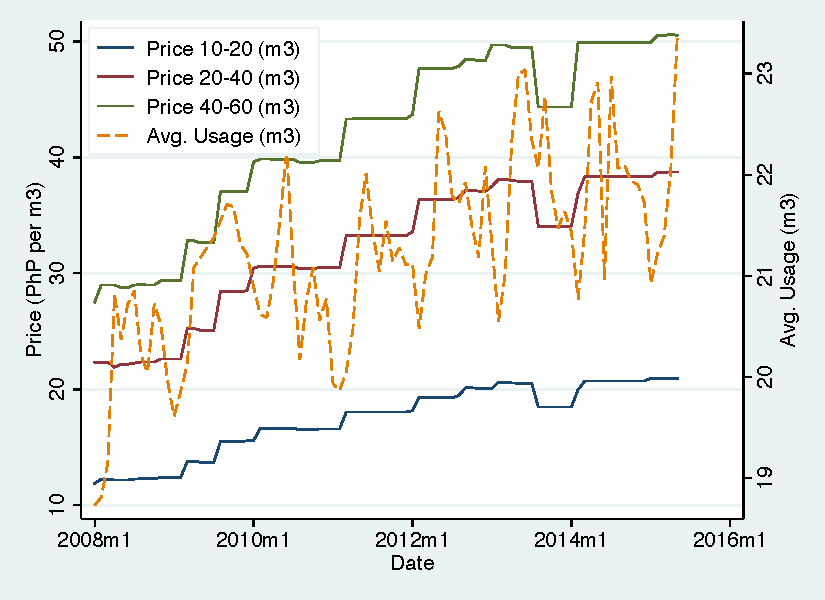
\includegraphics[scale=1]{tables/price_series.pdf}
\end{center}
\end{figure}


\begin{figure}
\caption{Tariff Schedule}
\begin{center}
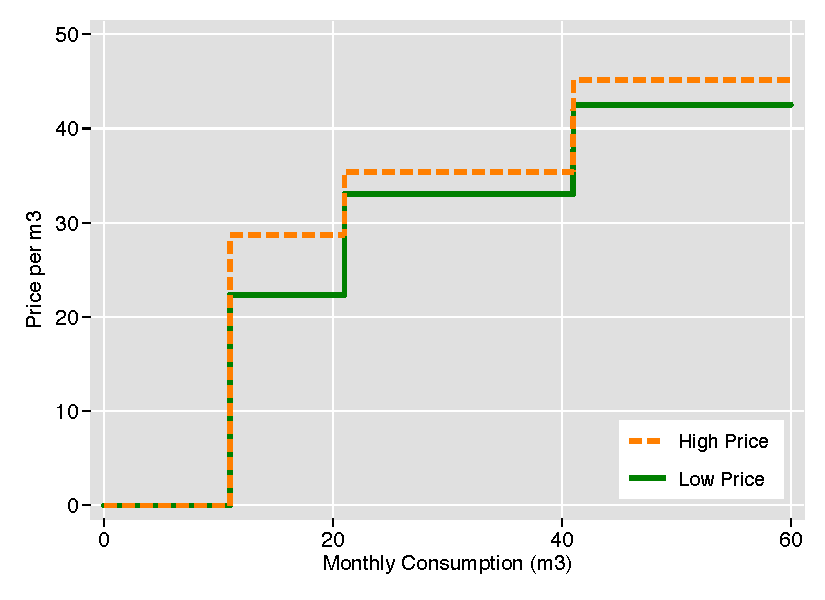
\includegraphics[scale=1]{tables/rs_prices.pdf}
\end{center}
\end{figure}

\begin{figure}
\begin{center}
\caption{Consumption Histogram}
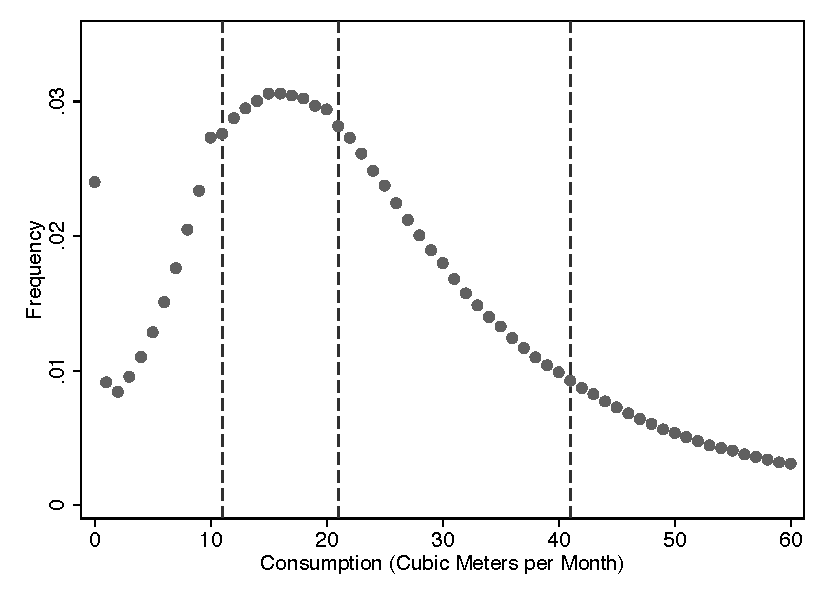
\includegraphics[scale=1]{tables/consumption_histogram.pdf}
\end{center}
\end{figure}


{
\small
\nocite{*}
\bibliographystyle{abbrvnat}
\setcitestyle{authoryear,open={((},close={))}}
\bibliography{library}
}



%\begin{center}
%  \input{mean_diff_leak1}
%\end{center}

%\begin{center}
%    \input{mean_diff_DC1}
%\end{center}



% \begin{table}[]
% \centering
% \caption{Source Choices}
% \label{my-label}
% \begin{tabular}{|l|c|c|c|}
% \hline
%                 & Fixed Price                  & Marginal Price                 & Tariff Kink Points      \\ \hline
% Individual (I)  & $F$                          & $P_k$                         & $\overline{w}_{k}$                         \\ \hline
% Shared   (S)    & $\frac{F}{2}$                & $P_k + P_{h}$                 & $\frac{\overline{w}_{k}}{2}$                            \\ \hline
% Vendor   (V)    & $0$                          & $P_{v}$                        & $0$                          \\ \hline
% \end{tabular}
% \end{table}
%\bibliography{lib}


\end{document}  